\section{Dataset}\label{dataset}

Per ottimizzare la costruzione di algoritmi predittivi, i dati di input vengono divisi in più set di dati con ruoli diversi. Tipicamente viene usata una specifica partizione dei dati in tre dataset: \textbf{training}, \textbf{validation} e \textbf{test set}.


\begin{defi}[Training set]
Il \textbf{training set} è un insieme di esempi utilizzati durante il processo di apprendimento per determinare (o imparare) le combinazioni ottimali di parametri.
\end{defi}

In pratica, è sui dati del training set che viene eseguito il metodo di ottimizzazione scelto, aggiornando quindi i valori dei parametri o degli iperparametri.

\begin{defi}[Validation set]
Il \textbf{validation set} è un set indipendente di dati usato per valutare il modello addestrato sul training set.
\end{defi}
La valutazione (o \textit{validazione}) del modello sul validation set porta a decidere quali siano i migliori valori per i parametri (o iperparametri) in base alla performance sul validation set, appunto. Nel caso dell'elaborato viene usato un early-stopper, che sceglie come miglior modello quello con minore errore subito prima che si verifichi overfitting.

\begin{defi}[Test set]
Un \textbf{test set} è un set indipendente di dati dal training set  usato solo per valutare le prestazioni del modello.
\end{defi}

\newpage

Cioè il test set viene usato per valutare su un terzo set di dati indipendente il modello scelto in base alla performance sul validation set. Si ottengono così caratteristiche di prestazione come la precisione, la sensibilità, la specificità... Questo dataset è importante perché permette di valutare la performance del modello su un terzo insieme di dati indipendente dai precedenti evitando il rischio di overfitting: se un modello addestrato sul training test si adatta anche al test set, si è verificato un overfitting minimo.

È stato più volte citato il problema dell'\textbf{overfitting}, viene quindi riportata la definizione.

\begin{defi}[Overfitting]
L'\textbf{overfitting} è la generazione di un modello (o un'analisi) che corrisponde troppo strettamente a un particolare insieme di dati e può quindi non riuscire a prevedere osservazioni future in modo affidabile.
\end{defi}

L'overfitting può verificarsi per esempio includendo troppi parametri regolabili o usando un approccio troppo complicato, come mostrato in figura \ref{overfittigComplex}. Chiaramente, quando si confrontano diversi tipi di modelli la complessità deve tenere conto dell'influenza di ogni parametro sull'output\footnote{Si noti che si può incorrere nel problema opposto usando un approccio troppo semplice: l'underfitting. Ad esempio cercando di approssimare con una regressione lineare un campione con un andamento parabolico.}.

\begin{figure}[htbp]
    \centering
    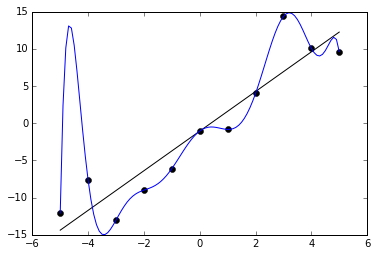
\includegraphics[width=0.6\textwidth]{images/Machine learning/Overfitted_Data.png}
    \caption{Esempio di overfitting. I dati (approssimativamente lineari) sono approssimati da una funzione lineare e da una polinomiale. Anche se la funzione polinomiale fornisce un adattamento quasi perfetto, ci si può aspettare che la funzione lineare generalizzi meglio i dati. \cite{wiki:overfitting}}
    \label{overfittigComplex}
\end{figure}

\newpage

L'overfitting è particolarmente probabile nei casi in cui l'apprendimento è stato eseguito troppo a lungo o in cui ci sono pochi dati per l'apprendimento, facendo sì che il modello si adatti a caratteristiche casuali molto specifiche dei dati di formazione che non hanno alcuna relazione causale con l'output. In questo caso di overfitting, la performance sul training set continua ad aumentare mentre la performance sul validation set peggiora, come mostrato in figura \ref{overfittingError}.



\begin{figure}[htbp]
    \centering
    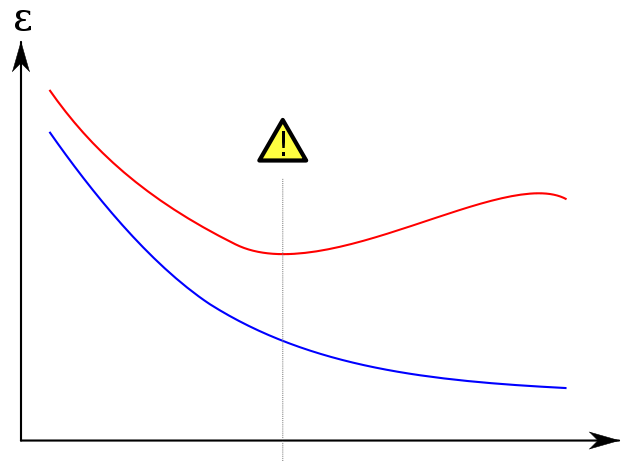
\includegraphics[width=0.6\textwidth]{images/Machine learning/Overfitting error.png}
    \caption{Overfitting nell'apprendimento supervisionato. Il training error (errore sul training set) è mostrato in blu, il validation error (errore su validation set) in rosso, entrambi in funzione del numero di cicli di training. \cite{wiki:overfitting}}
    \label{overfittingError}
\end{figure}


\subsection{Loss function}
Finora è stato delineato il problema che interessa l'elaborato: cercare una funzione $f$ per predire l'output $Y$ a partire dai valori dell'input $X$. Per farlo è necessaria una funzione di perdita, in inglese \textit{loss function}, $L(Y, f (X))$ per penalizzare gli errori di previsione.

\begin{defi}[Loss function]
Una \textbf{loss function} è una funzione in forma $\mathcal{L}(y_{\text{true}},y_{ \text{guess}})$ che definisce la perdita subita (o l'errore commesso) predicendo il valore $y_\text{guess}$ quando il valore vero è $y_{\text{true}}$,  fornendo quindi una valutazione delle capacità predittive del modello.
\end{defi}

Sarà questa la funzione da minimizzare con un algoritmo di ottimizzazione per l'adattamento degli iperparametri del processo gaussiano. Evidentemente la scelta della loss function dipende dal contesto.

%\section{Mean squared error}
%Per gli scopi dell'elaborato, si farà uso del \textit{mean squared error}.

%\begin{defi}[Mean squared error]
%Il \textbf{mean squared error} (o \textit{MSE}) è una \textit{loss function} definita come:
%\[
%\frac{1}{n}\sum^{n}_{i=1}(Y_i-f(X_i))^2,
%\]
%dove su $n$ dati raccolti, $Y_i$ sono gli output reali, $f(X_i)$ sono gli output predetti a partire da $X_i$.
%Poiché deriva dal quadrato della distanza euclidea, è sempre un valore positivo che diminuisce man mano che l'errore si avvicina a zero.
%\end{defi}
%Verrà usato non come loss function, ma per monitorare l'andamento del training.


%\section{Coefficiente di determinazione}
%Il coefficiente di determinazione fornisce una misura della bontà di adattamento di un modello, cioè quanto le previsioni di regressione approssimano i punti dei dati reali. Varia tra 0 e 1\footnote{Si possono apportare modifiche al coefficiente per fargli assumere anche altri valori, ma non vengono applicate nell'elaborato}, un $R^2$ di 1 indica che le previsioni di regressione si adattano perfettamente ai dati.

%Poichè il coefficiente di determinazione varia in un intervallo unitario, può essere più (intuitivamente) informativo di altre misure di errore (come il mean absolute error o il mean squared error) poiché tendono ad assumere valori su intervalli arbitrari oppure ad esprimere una percentuale.

%\begin{defi}[Coefficiente di determinazione]
%Date $y_i$ le osservazioni, $\overline{y}$ la media delle osservazioni, $\hat{y}_i$ i dati predetti dal modello:
%\[
%R^2 = 1-\frac{\sum_{i=1}^{n}(y_i-\hat{y}_i)}{\sum_{%i=1}^{n}(y_i-\overline{y})}
%\]
%\end{defi}
%Si noti che questo coefficiente non indica se:
%\begin{itemize}
%    \item una variabile sia statisticamente %significativa;
%    \item è stata usata la regressione corretta;
%    \item è stato scelto l'insieme più appropriato %di variabili indipendenti;
%    \item ci sono abbastanza dati per trarre una %conclusione solida.
%\end{itemize}

%Si noti inoltre che $R^2$ è una versione riscalata del mean squared error più facile da interpretare in quanto non dipende dalla scala dei dati.